%% 
%% Copyright 2007-2019 Elsevier Ltd
%% 
%% This file is part of the 'Elsarticle Bundle'.
%% ---------------------------------------------
\documentclass[preprint]{elsarticle}

\usepackage{graphicx}
\usepackage{tabularx,ragged2e,booktabs,caption}
\usepackage{tikz}
\def\checkmark{\tikz\fill[scale=0.5](0,.35) -- (.25,0) -- (1,.7) -- (.25,.15) -- cycle;} 
\usepackage[hyphens]{url}\urlstyle{same}
\usepackage{multirow}

\newcommand{\vale}[1]{\footnote{{\bf Valerio: #1}}}


\setcounter{tocdepth}{1}

\journal{Computer Communications}

\begin{document}

\title{A Review on Blockchain for the Internet of Medical Things: Definitions, Challenges, Applications, and Vision}

\author[1]{Gioele Bigini}%\fnref{fn1}}
\author[1]{Valerio Freschi}%\fnref{fn2}}
\author[1]{Emanuele Lattanzi\corref{cor1}}%\fnref{fn2}}
\ead{emanuele.lattanzi@uniurb.it}

\cortext[cor1]{Corresponding author}
%\fntext[fn1]{This is the first author footnote.}
%\fntext[fn2]{This is the second author footnote.}

\address[1]{Department of Pure and Applied Sciences, University of Urbino\\Piazza della Repubblica 13, 61029 Urbino, Italy}

\begin{abstract}
Disruptive innovation has led to the transformation of several sectors such as finance, automotive, and, lately, the healthcare sector.
Nowadays, there are lot of new devices that are increasingly capable of assisting healthcare professionals when working and helping people's well-being. 
This sector is getting benefit from the introduction of computer science but still clashes with the privacy and security regulations that, in healthcare, are particularly important.
In particular, lot of devices able to help people need the sharing of information to obtain better diagnoses results, but to date, there are no incentive systems for the use of these technologies which, for example, could reward the patients for the scientific contribution due to the sharing of their personal data.
 
A technology that promises to achieve this goal is the Blockchain which has spread widely following the success of Bitcoin, through its properties of decentralisation, immutability and transparency.
The Blockchain and the Internet of Medical Things can be considered to be at an early stage. Indeed, the applications actually working and applying successfully this technology are a few, and they mainly focus the attention on data sharing.
However, data sharing represents an interesting aspect to investigate, as well as interoperability of systems, security of devices and the opportunity to look for the monetisation of sharing through the blockchain. This review aims at giving an overview of the current state of the art of the blockchain-based systems for Internet of Medical Things, specifically addressing the challenges on the road for achieving more user centric systems, looking for a future potential direction.\\

	\begin{keyword}
	Blockchain \sep Internet of Medical Things
    \end{keyword}
\end{abstract}

\date{\today}
\maketitle

\section{Introduction}
The market has always turned its attention towards the impact of innovation. Over the past 30 years, the technology moved so quick steps that many of consolidated products and services have been replaced in order to provide better solutions: it is the age of disruptive innovation.
The role of computer science and engineering in this process is incontrovertible, forcing many industries to go along with it, often making it the company's core business, sometimes resulting in new products and services, but also new professions and improvements in an agile perspective of the industries.
In this fascinating context the Smart Health sector is rising, in some way, represented by the combination of computer science and healthcare with the goal of empowering professionals and addressing the well-being of people with innovative systems.

The healthcare sector has already enormously benefited from the introduction of computer science but much of the work still needs to be done, i.e. the sharing of information and the transition of system architectures from being system-centric to user-centric through decentralisation is still incomplete.
People using Internet of Medical Things solutions are actually involved in the sector but are not fully rewarded for their trust by the healthcare system except through performances coming from the usage of a service, despite the fact that their contribution is also scientific.
For example, every time we reach a doctor we contribute to the practical knowledge of the doctor himself. So, imagining to use a mobile Internet of Medical Things application this is still valid: using the application it is implicitly possible to contribute to something useful for the scientific sector that means giving free contribution at no cost.
Consequently, data from users represent a resource and should exist the possibility for him to choose what to give free, to hold or sell in the process.
Anyway, the are strong barriers represented by privacy and security for the health sector: the sharing of information without the explicit consent of the individual constitutes a strong violation of a person's rights.

A technology that promises to achieve this goal is the Blockchain, today one of the most discussed and debated tools of Information Technology (IT). 
The technology is presented as capable of changing the way how the IT systems are based, promising three fundamentals properties such as decentralisation, immutability and transparency. 
We will illustrate the advancements of the technology clarifying critical aspects for future implementations in the Internet of Medical Things.

Despite the multitude of applications in the Internet of Things sector, the narrower sphere of the Internet of Medical Things can be still considered to be in the early stages of its potential development. The word "Medical" wants to emphasise the specificity of these implementations. In fact, it should be specified that the sharing of information is not a general problem to address in all the practical applications, for example if the information processed by the devices does not constitute sensitive information then it is easier to find a way to share them, i.e. with techniques like anonymisation. But the drawbacks of these techniques is represented by the reduced amount of intrinsic information, that consequently could reduce the data exploitation.  
In a perspective in which medical information can lead to researches assisted by emerging analysis tools such as artificial intelligence, it is essential to respect the integrity of the data respecting the privacy, leading to the concepts of transparent management and data monetisation.

The main contribution of this review is to clarify the current state of the Internet of Medical Things, summing up those scientific papers that discuss this specific subset of the Internet of Things. We will discuss the technologies presented as capable of preserving privacy and security and the architectures currently conceived and/or implemented, with a look aimed at understanding the challenges for going forward a user centric solution and so, the future vision.

\section{Comparison to Other Surveys}

An increasing amount of works dealing with blockchain and IoT can be retrieved within current scientific literature, specifically pointing out opportunities for overcoming the challenges posed by security and privacy in the healthcare sector.
Based on this problem, an attempt has been made in this article to understand the research direction of the solutions based on blockchain architectures.

Searching on several databases as IEEE Xplore, Wiley Online Library, ACM Digital Library, MDPI, Springer and Scopus, with the keys "Blockchain" AND "Internet of Medical Things", 40 different works have been found. The lack of a bigger amount of papers shows that the field does not appear to be so investigated, thus confirming that the Internet of Medical Things, coupled with Blockchain, leaves room for more attention, researches and studies in the healthcare wider context.

Out of these 40 publications, 19 are survey papers discussing several challenges and opportunities posed by blockchain integration in the Internet of Medical Things. 
Here, researchers focus on addressing specific problems related to blockchain limitations or to give informative and procedural roadmap on how to start a Healthcare project on blockchain. Anyway, in this section we will classify papers basing on the macro areas they belong to as General Surveys, Problem Specific, Application Classification, eventually giving more detail where needed and what should be more investigated. 
In Table \ref{tab:reviewsclassification} the Review paper found are grouped in those sections. The reason for grouping this way the reviews reside on trying to quickly focus on the aim of the research made. The General Surveys section contain papers that talk about IoMT in a more informative way. Some researchers prefer to summarise theoretical problems specific to blockchain architecture for the healthcare (Problem Specific section) while others finally prefer to summarise real implementations of blockchain (Application Classification section).\\

\begin{minipage}{\linewidth}
\begin{tabular}{|p{6.84cm}|p{3.8cm}|}
 \hline
 \bf{Area} & \bf{Papers} \\ \hline
 	\multirow{4}{3cm}{General Surveys} 
     & \citet{pilkington2017can} \\
     & \citet{borovska2018big} \\
     & \citet{mackey2019fit} \\
     & \citet{agbo2019blockchain} \\ \hline
\end{tabular}
\begin{tabular}{|p{2.8cm}|p{3.6cm}|p{3.8cm}|}
 \hline
 \bf{Area} & \bf{Challenge} & \bf{Papers} \\ \hline
    \multirow{7}{3cm}{Problem Specific} 
    & Privacy and Security & \citet{nanayakkara2019security} \\
    \cline{2-3}
    & Data Management & \citet{banerjee2018blockchain} \\ 
    \cline{2-3}
    & \multirow{4}{4cm}{Frameworks for Blockchain-Based IoMT}
    	& \citet{fernandez2018review} \\
    	& & \citet{al2020intelligence} \\
    	& & \citet{pavithran2020towards} \\
    	& & \citet{chukwu2020systematic} \\ \hline
 	\multirow{8}{3cm}{Applications Classification}
 	& Scalability & \citet{mazlan2020scalability} \\
 	\cline{2-3}
 	& \multirow{2}{4cm}{Data Management and Interoperability}
 		& \citet{zhang2019review} \\
 		& & \citet{saha2019review} \\ 
 	\cline{2-3}
 	& \multirow{4}{4cm}{Healthcare Use Cases}
		& \citet{hussien2019systematic} \\
		& & \citet{holbl2018systematic} \\
		& & \citet{zubaydi2019review} \\
		& & \citet{khezr2019blockchain} \\ 
 	\cline{2-3}
 	& Industry Sectors & \citet{al2018blockchain} \\
 	\hline
\end{tabular}
\captionof{table}{Reviews Classification}
\label{tab:reviewsclassification}
\end{minipage}\\

\subsection{General Surveys}

\citet{pilkington2017can} and \citet{borovska2018big} addressed the growing segment of the Internet of Medical Things providing reflections on how these devices could contribute to big data, potentially leading to new medical solutions thanks to the application of machine learning techniques. According to their view, the intersection of big data analytics and precision medicine can be really promising for detecting diseases in the future.  They examined the blockchain technology as a medium for healthcare data management in general, considering the shortcomings of private and centralised organisations, analysing the transformative role of blockchain for the management of electronic health records.

\citet{mackey2019fit} and \citet{agbo2019blockchain} discussed the role of blockchains in facilitating data management, provenance and security, resulting into its potential to transform healthcare. They recognised that blockchain is not only about cryptocurrencies, but could be helpful in other sectors as healthcare. For example, the use of blockchain for privacy reasons on electronic health records, or for enabling credentials and licensing of medical professionals.%, or for advance in several fields of research such as the biomedical one. 
They also showed several examples of solutions based on blockchain in healthcare application scenarios which, however, generally lack of adequate prototype implementations. Hence, they highlighted the state-of-the-art in the development of blockchain applications for healthcare, concluding that there is still need of more research in the field to improve and evaluate the impact of the adoption of this technology.

\subsection{Problem Specific Reviews}
Data Management for the healthcare is extremely important because of the problems related to security and privacy. So, in a IoMT perspective this goal could be even worse to accomplish, since nowadays the mobile devices are generally more valuable for hackers to attack compared to other devices. 
In the reviews from \citet{khezr2019blockchain} and \citet{banerjee2018blockchain} the problems of Data Management in the Internet of Medical Things devices are addressed. Specifically, \citet{banerjee2018blockchain} consider the problem of keeping track of datasets on the blockchain as a way of data sharing. This is particularly interesting because they actually avoid the sharing of information directly on blockchain that actually is a strong barrier for implementation. In fact, it is actually difficult to think to a blockchain solution where data are stored on the blocks since the technology itself could not scale efficiently in size.

Privacy and security concerns are, needless to say, issues that go well beyond data management and blockchain. 
The review from \citet{nanayakkara2019security} consider several healthcare-based applications in the field of IoMT going through the threats and risks related to the field. The processing and sharing of information are not the only problems to face. The same devices, for example, in the IoMT could be tampered putting at risk the data of the individual. In this review the authors highlights how IoMT devices could be classified basing on the risks connected to them. They consider several technical risks as Middleware Threats, Application layer Threats, Business Layer Threats coming from the sensors that composed the medical devices.

Other researchers provided a kind of roadmap to approach a new project in the Internet of Medical Things domain based on blockchain. \citet{fernandez2018review} and \citet{al2020intelligence} focus the attention on the IoT context trying to set a framework to identify components and design elements for a new application in order to develop it. They consider specifically the blockchain as a medium to help cloud applications considering the IoT general architecture.

The review from \citet{pavithran2020towards} gives development plans for applications too. The authors focused on the roadmap to follow to build such kind of applications and to the identification of key factors and elements for the IoMT ecosystem. 
Specifically simulating two different types of blockchain implementation and discussing advantages in terms of throughput using device-to-device architectures instead of using gateway based implementations.

\citet{chukwu2020systematic} built their research using the Preferred Reporting Items for Systematic Reviews and Meta-Analysis (PRISMA) guidelines. They concentrated on the analysis of articles in order to discover privacy, security, cost, and performance issues, highlighting present frameworks and implementations. The conclusion of their investigation is that blockchain could be used in principle to solve the trust, security and privacy issues without sacrificing performances.

\subsection{Applications Classification Reviews}
Lots of researchers have taken into consideration the range of available applications to understand and better frame future directions and challenges.

Only one paper has been found addressing the scalability problems that blockchain generally pose (in every context not only the IoMT context), namely the review from \citet{mazlan2020scalability}. They suggest that in several cases the problem of scalability could be reduced in two main directions to take: storage optimisation and redesign of blockchain.

Data Management and Interoperability are hot topics for IoMT and a priority for the healthcare sector in general. The review from \citet{zhang2019review} summarises the existing blockchain-based systems and applications, classifying them by traceability and data security protection and trying to understand opportunities and challenges for the development in the industry. 
\citet{saha2019review} analysed the ability of blockchain systems to support data integrity, reliability and the capability to address security issues of the cloud. Specifically, they worked on medical data sharing and storing with blockchain-based cloud and investigated the current state-of-the-art on blockchain-based medical healthcare system discussing several works in the domain.

For what concerns the use cases in the healthcare domain, \citet{hussien2019systematic}, \citet{holbl2018systematic}, \citet{zubaydi2019review} and \citet{khezr2019blockchain} conducted their reviews by analysing the use of blockchain in healthcare applications and putting them into a coherent taxonomy. Their work provides insights on the increasing number of studies related to the adoption of blockchain technology, looking for several motivations as data sharing or security issues between healthcare providers, by pointing out the potential role in revolutionising the healthcare industry.

Finally, \citet{al2018blockchain} investigated the Internet of Things, healthcare, supply chain management, and government sectors and for each sector they described the use cases in which an attempt is made to implement blockchain solutions. They found out the growing maturity, benefits and challenges of blockchain technology underlining the need for further investigations at that time, for all the sectors involved.

\subsection{Our Position} 
In this review we would like to move the attention over the Internet of Medical Things solution centered on final users, something that we find out is not deepened in any review. We will go through the current challenges for the Smart Health applications to be coupled with blockchain in order to move forward an idea of blockchain-based implementations in which the system should be independent from the Healthcare providers and more user-centric (or patient centric, describing it from the medical position).

\section{Healthcare and Internet of Things: Privacy and Security Issues}

A typical Internet of Things (IoT) infrastructure is made up of several devices connected to the Internet able to communicate each other. The most widely diffused and known devices that can be considered a building block of the IoT ecosystem are the smartphones. In general, any electronic device that has the capability of interfacing to and communicate with other nodes of the Internet can be considered part of the IoT network, for example home automation systems or voice recognisers. 

The ability to communicate each other on the Internet clearly poses important security and privacy issues, for example: a voice recogniser needs more interaction with the user and to be listening to improve its learning, while a home automation system could be hacked by a malicious user getting the access to important functions of the smart home solution.

Therefore, the context in which the devices operate is fundamental for understanding the rules to follow in terms of privacy and security. For the specific subset of the Internet of Medical Things, the sensitivity of the users data and the vulnerabilities of the devices themselves represent serious problems. If the devices need to exchange information on the network, they could be a perfect target to hit. A typical solution used to avoid information leakage is to move all the processing onboard of the device (avoiding data transmission on the network) or transferring information only once masked or anonymised, definitely impacting on data quality and integrity too. 

So, from one side processing data on the device limits the risk of information leakage by malicious users but at the cost of performances, while the anonymisation technique tries to irreversibly prevent identification but at the cost of part of the data. This implicates extensive stripping of data and largely excludes data linkage and update, sometimes essential activities for the Internet of Medical Things \cite{mostert2016big}.

\section{Blockchain}

\begin{figure}[tph!]
	\centering
    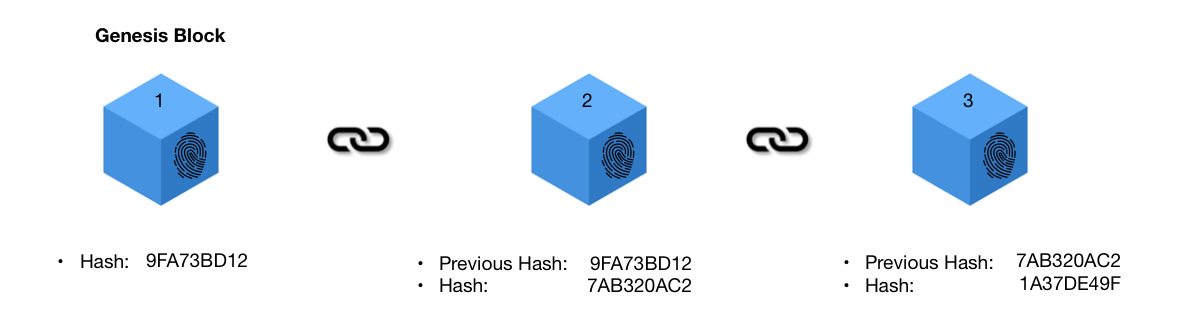
\includegraphics[totalheight=3cm]{img/bck_chain}
    \caption{Blockchain Technology Example}
    \label{fig:blockchain}
\end{figure}

The term "Blockchain" refers to a technology discussed for the first time over 20 years ago, often confused with Bitcoin \cite{nakamoto2008bitcoin} (and vice versa) which represents the first successful attempt to apply the technology. Blockchain is presented as a technology able to provide decentralisation, immutability and transparency.

From a purely technical point of view, the Blockchain has not brought anything new: all the elements for its implementation have been known for years. However, from a conceptual point of view it could constitutes a real revolution. Through the Blockchain, to which this name has been attributed due to its block chain structure, the distribution of information is guaranteed in a decentralised manner, therefore in the absence of a central entity, avoiding any tampering or, better, minimising it to a point that makes it a negligible possibility.

The birth of the concept comes from Stuart Haber and W. Scott Stornetta in 1991 through their paper ``How to time stamp a digital document''\cite{haber1990time} from which practically all ideas are collected. Blockchain is a growing list of data structures, called blocks, connected and secured through encryption.

A block of the Blockchain can potentially contain any type of information in addition to that intended as mandatory. For example, to form a chain of blocks it is necessary to know the previous and the next element. In the particular case of the Blockchain, this link between a block and its previous one is given by a Hash. The choice is not random at all and wants to find correspondence with fingerprints, that is, it is an identification method without this leading to the characteristics of its bearer.

The chain originates from a single block, called ``Genesis Block''. The content of the blocks can be anything depending on the purpose of the project itself and it can be readable or not depending one the access to the blockchain. This case can be explained classifying blockchains between ``Permissioned'' and ``Permissionless'' blockchains, in which access to the chain is managed by a central entity. This fact also impacts on decentralisation and will be later discussed as well as the concept of ``Public'' and ``Private'' blockchains. 

Implementations of any kind actually exists, exploiting several advantages. In this review, however, we will try to give a deep understanding of what actually means to give trust to different implementation of Blockchains. It is convenient to mention, in fact, that the most ``pure'' versions of Blockchain (e.g. the one from Bitcoin) are actually founded on concepts as: Hash Encryption, Immutable Ledger, Distributed P2P Network, Mining, Consensus Protocol. Nonetheless, these properties are in general not adopted as a whole by all solutions proposed.

\subsection{Public and Private Blockchains}
Public blockchains are built in a way to avoid control by any central entity on the network. This means that if peers in the network trust the technology, the blockchain constitutes a distributed network sharing a cryptographic secure immutable ledger accessible to anyone. The ability to add blocks on the chain is guaranteed by a consensus protocol, a mechanism defined for the specific blockchain through which the participants converge to reach consensus (the most famous is Proof-Of-Work implemented by Bitcoin first \cite{back2002hashcash}). This is the best way to exploit blockchain in all its capabilities and they are often referred as ``Permissionless'' since there is free access to blocks content across the network.

Private blockchains are restricted to providers that determines various level of access. This kind of implementation basically sacrifices decentralisation for a restricted control over the blockchain itself. It can be useful in those cases in which there is a need of having only some actors participating on adding blocks to the network for various reason. It can be both ``Permissioned'' or ``Permissionless''. Anyway, in the case of a permissioned environment, the technology differs from the original vision of blockchain technology since the blocks are not freely accessible but have a small group of actors who can access it and not only that, since the participants are very limited the blockchain could not need a consensus protocol, an example of this is IBM Hyperledger \cite{androulaki2018hyperledger}.

\subsection{On-Chain and Off-Chain Transactions}
Off-chain transactions refer to those transactions occurring on the blockchain which move the value outside of the blockchain. This is possible by several behaviours as swapping private keys of existing wallets or by using a third-party or coupon-based interlocutor. This can lead to no fees, immediate settlement and full anonymity without recording anything on-chain. Moreover, this kind of transactions can be always reversed if no operation has been done on-chain. In contrast, an off-chain transaction takes the value outside of the blockchain. It can be executed using multiple methods. First, there can be a transfer agreement between transacting parties. For example, coupon-based payment mechanism are based on off-chain methods: a participant purchases coupons in exchange for the crypto-tokens, and gives the code to another party which can then redeem them.

On-chain transactions refer to those transactions which occur on the block-chain, the usual interpretation of cryptocurrencies transfer so when the transaction is put in a block and validated by miners. Depending upon the network protocol, once a transaction gains enough confirmations from network participants it becomes irreversible. To reverse it, it would mean to be able to tamper the blockchain. On-chain transactions are supposed to occur in pseudo real-time because new blocks are broadcasted and added to the blockchain. This broadcasting need make the transactions not to occur instantly since the information needs to reach the whole network and to reach a proper consensus. They also come at a cost, as miners ask for a fee for their transaction confirmation on the blockchain in the shortest possible time. The fee in some way determines the rapidity of the response since miners could look for highest fees.

\section{InterPlanetary File System}
The InterPlanetary File System (IPFS) is a peer-to-peer distributed file system that seeks to connect all computing devices with the same system of files \cite{benet2014ipfs}.
 
The IPFS was born by looking to the data sharing platforms of the past: Napster for example that basically were large file distribution systems supporting over million of users. However, the applications were not designed as infrastructure to be built upon, i.e. as a general file-system that offers global, low-latency, and decentralised distribution.

Moreover, industries where initially interested in such kind of systems because the network was slower and moving files across the network was relatively difficult. Instead, with the advent of wide bandwidths HTTP did greatly its job.
Anyway, there are several challenges that could appear again as:
\begin{itemize}
	\item Hosting and Distributing;
	\item Versioning and linking of massive datasets;
	\item Computing on large data across organisations;
	\item High-volume at High-definition on-demand or real-time media streams.
\end{itemize}
This challenges will be a reality in the future and IPFS provides a high throughput content-addressed block storage model solution with no single point of failure where nodes do not need to trust each other.

\section{Security and Privacy Regulations}
In several region of the world, there are different laws to respect concerning privacy and security. For example, in Europe all private companies and public bodies have been obliged to comply with the new European legislation on the protection of personal data (General Data Protection Regulation \cite{gdpr2016eu}). 

In the health sector, all healthcare providers such as hospitals and research centers have transformed the way they work in order to avoid the possible sanctioning consequences by not respecting the new regulation.

For the specific case of health data handling, sources as ``genetic data'', ``biometric data'' and ``health data'' must be managed carefully. These data are traced back to the sensitive category and so, they cannot be used without explicit consent unless for some cases as preventive or occupational medicine, diagnoses, assistance, health therapy and reasons of public interest (only for the public health sector). The same happens to data portability which basically also place constraints on how data is shared.

Moreover, all public authorities, bodies and all those private individuals who, as main activity, carry out regular, systematic and large-scale monitoring of people health data must designate a professional figure who, through his skills, is employed in data protection.

\section{Scientific Papers Review}
Complete implementations of Internet of Medical Things systems based on Blockchain, or in some way assisted by the technology, are not so many and indeed they should need more investigations. 
This is supported by the fact it is estimated that by 2026 there will be a dramatic increase in IoMT systems of about 140 billion dollars \cite{fortune2020iomt}. In Table \ref{tab:scientificpapers} we give a classification of those trying to focus on the kind of solutions and their degree of decentralisation with the final goal of giving an information about the centricity of the user on the whole architecture.\\

\begin{minipage}{\linewidth}
\begin{tabular}{|l|p{3.25cm}|p{5.2cm}|}
 \hline
 \bf{Publication} & \bf{Focus Area}  & \bf{Papers} \\ \hline
 	\multirow{12}*{Theoretical} 
 	&  
 	\multirow{10}*{Framework for IoMT} 
 		& \citet{shae2017design} \\
 		& & \citet{angeletti2017role} \\
 		& & \citet{alblooshi2018blockchain} \\
		& & \citet{bhawiyuga2019platform} \\
		& & \citet{chakraborty2019secure} \\
		& & \citet{seliem2019biomt} \\
		& & \citet{nguyen2019blockchain} \\
		& & \citet{abdellatif2020sshealth} \\
		& & \citet{firdaus2018root} \\
		& & \citet{dwivedi2019decentralized} \\
 	\cline{2-3}
 	& \multirow{2}*{IoMT Security} 
 		& \citet{meng2019enhancing} \\
 		& & \citet{srivastava2019data} \\ \hline
\end{tabular}
\end{minipage}

\begin{minipage}{\linewidth}
\begin{tabular}{|l|p{3.25cm}|c|p{2.7cm}|}
 \hline
 \bf{Publication} & \bf{Area} & \bf{Type} & \bf{Work} \\ \hline
 	\multirow{12}*{Applications}
 	& \multirow{6}{3.25cm}{Data Management and Interoperability}
 	& Mixed & \citet{jiang2018blochie} \\
 	\cline{3-4}
 	& & Mixed & \citet{xu2019healthchain} \\
 	\cline{3-4}	
 	& & Centralised & \citet{wang2019blockchain} \\
 	\cline{3-4}
 	& & Centralised & \citet{dey2017healthsense} \\
 	\cline{3-4}
 	& & Centralised & \citet{azbeg2018blockchain} \\
 	\cline{3-4}
 	& & Centralised & \citet{nguyen2019mobile} \\
 	\cline{2-4}
 	& Alerting System & Centralised & \citet{jo2018hybrid} \\ 
 	\cline{2-4}
 	& \multirow{5}{3.25cm}{Data Crowdsourcing}
 	& Decentralised & \citet{fernandez2019enabling} \\
 	\cline{3-4}
 	& & Centralised & \citet{rupasinghe2019towards} \\
 	\hline
\end{tabular}
\captionof{table}{Scientific Papers Classification}
\label{tab:scientificpapers}
\end{minipage}\\

%\citet{dilawar2019blockchain} &  \checkmark & \\ \hline
%\citet{xu2019healthchain} &  \checkmark & \\ \hline
%\citet{srivastava2019light} &  \checkmark & \\ \hline
%\citet{ahram2017blockchain} & \checkmark &  \\ \hline	
%\citet{kumari2020securing} & & \checkmark \\ \hline

In the following sections we will analyse in deep the scientific papers trying to understand the current state of the research for blockchain-based system with a user-centric architecture. As the classification shows, actually building a fully decentralised solutions seems not so investigated. This particular problem will be underlined in the following, keeping an eye into the future.

\subsection{Data Management and Interoperability}
As mentioned throughout this review, the data sharing issues are actually highly interesting from a medical point of view. The possibility of freely sharing sensitive information between professionals and health institutions would allow a great leap forward from the point of view of research in the medical field, taking advantage of the most advanced machine learning techniques that computer science is offering.

There are several way of thinking on how to share data on the blockchain: storing data in its blocks (even if this seems very difficult actually due to scalability issues) or using it for data provenance that basically means storing positions of data in the blockchains instead of data itself. So, in the latter case, data is never moved within the network, rather it is accessed knowing its position during time.

Right now, data sharing is a huge barrier for interoperability that needs to be solved in such a way that users can be masters of their data.

\citet{nguyen2019mobile}, \citet{dey2017healthsense}, \citet{azbeg2018blockchain} and \citet{nguyen2019mobile} focus on the safe transmission of healthcare data. They specifically focus on cloud-based IoMT devices used for monitoring disorders finding in the blockchain a safe system for data sharing between devices through the help of smart contracts. 

A step through interoperability have been made by \citet{jiang2018blochie} and \citet{xu2019healthchain} through a solution more prone to decentralisation. Both of them tried to reach a major decentralisation by using a combination of different blockchains achieving different scopes.

\subsection{Alerting Systems}
We find out a specific case from where data are used for creating an alerting system. The actual system could not be considered decentralised since it requires smart contracts in order to work but the final result is interesting: the idea that we can trust transparent and immutable code. \citet{jo2018hybrid} build a IoT with blockchain-based smart contracts for Structural Health Monitoring of underground structures using smart contracts as a transparent tool to spread alerts. Even if the smart contract acts as a centralised resource the fact that it is actually immutable puts it in a trustable, transparent and verifiable condition. 

\subsection{Data Crowdsourcing}
Some researchers focus on the hypothesis that the blockchain can actually be a new way of doing crowdsourcing with monetisation. \citet{fernandez2019enabling} and \citet{rupasinghe2019towards} build a centralised solution based on smart contracts for achieving this goal.

\subsection{Classification by User Centricity}
A further classification that distinguishes the problem faced and the Blockchain proposed for each of them can be well defined. A classification by user centricity means trying to understand if the user is able to get full control on his data or not. IoMT systems generally rely on a centralised entity through which they give a service, this seems to happen even with the Blockchain. However, a user centric system could be a lot useful in such a context and for this reason we try to give a classification of the papers based on this.

In essence, a user-centric solution is a way of seeing the blockchain-based solution as able to give to the participant the ability of no longer need a central provider to take care of the data. This goal should enable worldwide interoperability too. As shown in Table \ref{tab:classification}, for each analysed application there is no solution able to fully put the user in a distributed and decentralised position that means that this topic needs more investigation.\\

\begin{minipage}{\linewidth}
\begin{tabular}{|p{3.5cm}|l|l|c|}
 \hline
 \bf{Application} & \bf{Paper} & \bf{Centricity} \\ \hline
 \multirow{6}{3.5cm}{Data Management and Interoperability}
 	&
 		\citet{jiang2018blochie} & System \\ \cline{2-3}
 	& 
 		\citet{xu2019healthchain} & System \\ \cline{2-3}
 	& 
 		\citet{wang2019blockchain} & System \\ \cline{2-3}
 	& 
 		\citet{dey2017healthsense} & System \\ \cline{2-3}
 	& 
 		\citet{azbeg2018blockchain} & System \\ \cline{2-3}
 	& 
 		\citet{nguyen2019mobile} & System \\ 
 	\cline{1-3}
 	
 Alerting System 
 	& 
 		\citet{jo2018hybrid} & System \\ \hline
 \multirow{2}*{Data Crowdsourcing}
 	& 
 		\citet{fernandez2019enabling} & System \\ \cline{2-3}
 	& 
 		\citet{rupasinghe2019towards} & System \\ 
 	\cline{1-3}
\end{tabular}
\captionof{table}{Application Classification}
\label{tab:classification}
\end{minipage}\\

% \citet{dilawar2019blockchain} & Communication Security & \checkmark & \\ \hline
% \citet{nguyen2019mobile} & Data Sharing & \checkmark & \\ \hline
% \citet{nguyen2019blockchain} & Data Sharing & \checkmark & \\ \hline
% \citet{meng2019enhancing} & Medical Smartphones Security & \checkmark & \\ \hline
% \citet{firdaus2018root} & Medical Devices Security & \checkmark & \\ \hline
% \citet{ahram2017blockchain} & Blockchain for Healthcare & \checkmark & \\ \hline	
% \citet{kumari2020securing} & Communication Security & \checkmark & \\ \hline
% \citet{ilinca2020applying} & & & \\ \hline	

\section{A User-Centric Perspective for the Internet of Medical Things}
In the reviews found is strong the need of creating a user-centric approach, where the user has full control over her/his data, in order to reach a transparent interoperability. Several attempts have have been made to solve this problem but still they do not offer a final solution that completely goes forward this direction. What we just highlighted can be further clarified with the considerations that follow.

\citet{jiang2018blochie} propose a platform named BlocHIE based on blockchain for data sharing between individuals employing two Blockchains, namely EMR-Chain for medical institutions and PHD-Chain for individuals, both able to submit and share healthcare data. They handle healthcare data through the combination of off-chain storage and on-chain transactions. The off-chain storage is achieved by storing the data in the distributed databases of the hospitals while the on-chain verification is achieved by including the hash value of each medical record in the transaction. 
Because medical institutions usually submit very privacy-sensitive data as medical reports and treatments (because of healthcare professionals) while individuals are more prone to submit huge amount of data (because of data generated by IoMT devices), such kind of approach provide from one side a centralised solution where institutions are able to keep control of user data and to the other side a decentralised solution for data provenance. The whole system could then be considered as a mixed solution between centralisation and full decentralisation but still system centric.
	
\citet{xu2019healthchain} propose Healthchain, a large-scale health data management scheme based on blockchain where users have full control of their data as well as access policies. The system use two blockchains namely Userchain, a public blockchain used to publish users' data, and Doccchain, a private blockchain of healthcare institutions used to publish doctors diagnoses. For the researchers this scheme should ensure the design goals of supporting large-scale IoT devices, reaching a high efficiency, and creating a real-time online diagnosis system, which could preserve privacy, ensure accountability and, finally, manage permissions. 
It is composed of five entities: the IoT Devices; the User Nodes, able to manage one or more IoT devices aggregating, encrypting and sending data to the storage node; the Doctor Nodes that are doctors or companies providing healthcare services; the Accounting Node: a special node maintained by the consortium to verify whether the transactions from doctor nodes are correct and valid; Storage Nodes, IPFS-based systems maintained by the consortium that collaboratively store complete encrypted users' IoT data and encrypted doctors' diagnoses in a distributed manner. 
Basically, IoT devices send health data to the User Nodes that encrypts the data forwarding them to an IPFS storage that takes care of the transaction to the Userchain. The Doctor Node is then able to give real-time online diagnoses readable by patients reading the Docchain.
	
\citet{wang2019blockchain} propose a blockchain-based eHealthcare system using Hyperledger Fabric interoperating with wireless body area networks (WBAN) which utilises the WBAN to network the devices of the patients and the blockchain technology as the data management system. Hyperledger Fabric provides a private, permissioned network where participants trust each other. The actors of such a system are: patients, doctors, healthcare institutions and suppliers. 
The workflow of the proposal is the following: the patients transmit the data collected through the WBAN from the sensors to the centralised devices. The devices wait for the instructions by the centralised device that later generate the final record of information to submit to the blockchain, in order to update the physical data of the patients. 
In this kind of architecture, the data are effectively kept safe: healthcare professionals get access only to the records of their patients. Anyway, Hyperledger Fabric cannot be considered as a pure blockchain because fails to deliver one the most important feature of the blockchain: the decentralised consensus. In this sense, Hyperledger Fabric does not require any consensus mechanism at all making difficult to know if it the ledger has been tampered \cite{cointelegraph2019ibm}.

\citet{dey2017healthsense} propose a blockchain-based model where a sensor collects real time data of a patient medical condition and stores it in the blockchain for later use with smart contracts. The solution make use of IPFS for off-chain storage and through a smart contract te sensor is put in communication with the blockchain. In some way, this allows IoMT devices to autonomously find each other and begin trading data off-chain or with the platform. 
The model proposed lack of solution for mining and so, does not allow sensors to add new blocks to the blockchain (that are considered low power). In this configuration, the model could be still system centric and permissioned, with no decentralisation.
 	
\citet{azbeg2018blockchain} propose a platform architecture based on a permissioned Blockchain for diabetes self-management. The researchers said that integrating Blockchain with low power devices, such as the ones used for diabetes monitoring is a difficult task. 
The way they reached this goal was by registering each new device in the blockchain by its owner, the one able to gave permission to access the blockchain. So the system is composed by the devices, the blockchain and the medical institutions (that maintains the blockchain). 
The connection to the blockchain is realised through a gateway (a smartphone) able to encrypt and route information to an off-chain IPFS database which can be accessed by authorised physicians and healthcare teams. The healthcare institutions are actually the full nodes of the network: they store pointers to data, validate transactions and create new blocks as other similar centralised solutions.
 	
\citet{nguyen2019mobile} propose a dataset sharing system for an IoMT infrastructures composed by mobile devices and cloud technologies. Their idea is to focus on the integrity of the datasets available for download, making them available for sharing.  They developed an access control mechanism through smart contracts and delegated to a central hub the repositories maintenance of the datasets, while distributed keeping information such as the address, ownership and sharing policies on the blockchain. The blockchain is public and does not contain sensible data. Moreover, this attempt is interesting because the owner of the dataset can remove the data in any moment, making them not accessible anymore. However, in this way the blockchain could have several blocks with ``empty links'' (stored as transactions). %that could results in an uncomfortable situation.
 	
\citet{jo2018hybrid} proposed a simulation for autonomous monitoring and control of structures through blockchain-IoT network. The proposed structure of blockchain is private and permissioned to allow only the authorised parties the interaction. 
The proposed architecture is mainly composed of core and edge networks where the blockchain acts as a distributed ledger for collecting occurrences of events in the form of transactions. Smart contracts are responsible of sending alerts, that are recorded as a completed transaction in the core blockchain network. Edge nodes serve as a centralised server for the real-time response of inquiries and offer low latency and bandwidth usage. Edge nodes hold access control mechanisms and contain the signature keys of participants.
To ensure the integrity of data in the core network, the generation of new blocks is assigned to participants that acts as miners with a proof-of-work (PoW) consensus protocol. Anyway, in a private and permissioned blockchain the risk of tampering is higher than a public and permissionless because of lower participation level.

\citet{fernandez2019enabling} proposed a system for monitoring patients remotely and warning them about potentially dangerous situations. It uses smartphones to collect information and sends them to a remote cloud or to distributed fog computing nodes. In order to exchange data between healthcare parties the system includes the deployment of a decentralised storage system that receives, processes and stores the collected data and provide a criptocurrency as an incentive for participation. 
The architecture consists in an interface for users that allow the access of the stored information; a decentralised storage system that replicate the collected information and distribute it automatically among multiple nodes; a distributed ledger that use smart contracts in order to reward participation. This kind of approach is interesting and goes toward data crowdsourcing with blockchain.
 	 	
\citet{rupasinghe2019towards} propose a conceptual blockchain based fall prediction model using smart contracts and the FHIR (Fast Healthcare Interoperability Resources) standard protocol. They identify four roles: person under care, primary care provider (or long term provider), secondary care provider (or short term providers) and temporary care giver. Each of these entities are maintaining their own electronic health record management systems and can be considered as data sources for the final prediction model.
The architecture is based on a permissioned and private blockchain that leverage on smart contracts for accessibility, creating different access levels based on each user category. 

\section{Remarks and Future Directions}
The review focused on the ability of blockchain of creating specific solutions able to enable user (specifically for the healthcare sector patients) to be the true owner of their data. At the moment, what is evident is the lack of solutions oriented to user-centricity. There are several solutions that are able to grant interoperability but the problem of user centricity still remains as well as weak security and privacy. What this review underlined is how these problems could be solved together, potentially paving the way to deal with the problem of data management for the healthcare.
 
Moving the architectures from a system centric system, where a user is the consumer of the application, to a user centric system, where the user is more than a consumer but an active participant, basically consists in moving to a blockchain economy, that is to say: networks as a medium of active contribution to a community, as the one of the healthcare. This could be more interesting when these networks can reward the participants and able to interact each other.

This vision also settles very well with a concept that has been found in one review only: rewards for data contribution. As said previously, whenever an individual uses an IoMT system or an IoT device, it is never rewarded for the contribution it makes. Normally individuals pay to get a professional help but their contribution is higher than the mere performance received. In fact, in principle, they could also contribute to enhance scientific knowledge. Today, this information is basically lost by not contributing or, when it occurs, does not mean reward. In an increasingly Blockchain-enabled world, the Internet of Blockchains could definitely enable data sharing, or data crowdsourcing.

\section{Conclusions}
The wellbeing is the foundation for the lifestyle of a healthy individual and managing medical data could help users on achieving the goal. 

In the past the need for large amount of data and privacy issues were not considered: the traditional method for data collection was through recordings on paper, medical science was not supported by actual technology usually leading to no explanation for several diseases and no solution. Quickly with the introduction of technology has been clear how it was possible to deliver and discover new solutions and how much the data collected by patient monitoring where useful for him and for the healthcare community. By introducing the Internet of Medical Things potentially any data collected by a user could be exploited with a specific goal. 

We examined in this work the contributions of the blockchain to IoMT applications, focusing on the current challenges and vision for the future. The review aimed in particular at summarising scientific articles that attempt to understand the state of the industry from a practical point of view and which are the related problems that currently act as barriers for a subsequent step forward user centricity. 

Several papers have been investigated focusing on their approach towards interoperability with blockchain, assessing which of those were supporting the idea of data crowdsourcing with blockchain in user centric manner. Blockchain is finally a true candidate to bring a radical change in the healthcare data management solutions. Through the achievement of specific objectives such as security, scalability and interoperability, the blockchain can be the driving technology through which to develop lasting and independent platforms for data sharing that can give value to privacy.

\section*{Bibliography}
%\nocite{*}
\bibliographystyle{elsarticle-num-names}
\bibliography{bibliography}

\end{document}

